\documentclass{extbook}
\usepackage[papersize={8.5in,11in},top=1in,bottom=1in]{geometry}
\RequirePackage{fix-cm}
\usepackage[T1]{fontenc}
\usepackage{lmodern}
\usepackage{fullpage}
\usepackage{titlesec}
\usepackage{parskip}
\usepackage{float}
\usepackage{url}
\usepackage{hyperref}
\usepackage{graphicx}
\usepackage{listings}
\usepackage{tcolorbox}
\usepackage{tabularx}
\usepackage{xcolor}
\usepackage{titlesec}
\usepackage{amsmath}
\usepackage{pdfpages}
%\usepackage{fancyhdr}

%renombro de ingles a español
\renewcommand{\contentsname}{Contenido}
\renewcommand{\figurename}{Figura}
\renewcommand{\listfigurename}{Lista de figuras}
\renewcommand{\bibname}{Bibliografía}
\renewcommand{\tablename}{Tabla}
\renewcommand{\listtablename}{Lista de tablas}


\usepackage[fontsize=13.5pt]{fontsize}
\setlength{\parindent}{0pt}

\titleformat{\chapter}[display]
  {\bfseries\huge} % Estilo del título
  {\hfill\Large} % Alineación a la derecha
  {3ex} % Espaciado entre el número del capítulo y el título
  {\vspace{-5cm}\titlerule\vspace{1.5ex}\hfill} % Regla arriba y alineación del título a la derecha
  [\vspace{1ex}\titlerule] % Regla debajo del título


  \makeatletter
  \patchcmd{\chapter}
    {\if@openright\cleardoublepage\else\clearpage\fi}
    {\clearpage}
    {}{}
  \makeatother

  \definecolor{codegreen}{rgb}{0,0.6,0}
  \definecolor{codegray}{rgb}{0.5,0.5,0.5}
  \definecolor{codepurple}{rgb}{0.58,0,0.82}
  \definecolor{backcolour}{rgb}{0.95,0.95,0.92}
   
  \lstdefinestyle{mystyle}{
      backgroundcolor=\color{backcolour},   
      commentstyle=\color{codegreen},
      keywordstyle=\color{magenta},
      numberstyle=\tiny\color{codegray},
      stringstyle=\color{codepurple},
      basicstyle=\footnotesize,
      breakatwhitespace=false,         
      breaklines=true,                 
      captionpos=b,                    
      keepspaces=true,                 
      numbers=left,                    
      numbersep=5pt,                  
      showspaces=false,                
      showstringspaces=false,
      showtabs=false,                  
      tabsize=2
  }
   
  \lstset{style=mystyle}
\setcounter{secnumdepth}{4}
\setcounter{tocdepth}{3}
\mainmatter
\setcounter{secnumdepth}{4}

\begin{document}
\thispagestyle{empty}
\begin{minipage}{.15\textwidth}
  \flushleft
  \center{
\includegraphics[scale=0.035]{Imagenes/utp.png}}

  \vspace{20pt}

  \center{
    \rule{.5pt}{.6\textheight}
    \hspace{7pt}
    \rule{2pt}{.6\textheight}
    \hspace{7pt}
    \rule{.5pt}{.6\textheight}
  } \\

  \center{
\includegraphics[scale=0.28]{Imagenes/fisc.png}}
\end{minipage}
\begin{minipage}{.7\textwidth}
\flushright

\center{
  \center{
    \LARGE{U}\large{NIVERSIDAD} 
    \LARGE{T}\large{ECNOLÓGICA} \\[10pt]
    \large{DE} 
    \LARGE{P}\large{ANAMÁ} 
  } \\
  \rule{\textwidth}{2pt}
  \\
  \hrulefill\\[.5cm]
  
  \center{
    \LARGE{F}\large{ACULTAD DE } \LARGE{I}\large{NGENIERÍA} \LARGE{D}\large{E}\\[0.35cm]
    \LARGE{S}\large{ISTEMAS} \LARGE{C}\large{OMPUTACIONALES}\\[1cm]

    \LARGE{C}\large{ENTRO} \LARGE{R}\large{EGIONAL} \LARGE{D}\large{E} \LARGE{V}\large{ERAGUAS}\\[1cm]

  }


  \rule{\linewidth}{0.75mm}\\
  {\Large \textsc{Prototipo de cubo de basura inteligente con Detección de Material y Monitoreo de Llenado basado en Arduino y ESP32 para la Universidad Tecnológica de Panamá}}\\[0cm]

  \rule{\linewidth}{0.75mm}\smallskip

  \large{PRESENTA:}\\[0.3cm]

  \large{ \textbf{BARRERA, ARLAND\\[0.2cm]
  ORTEGA, PRISCILA\\[0.2cm]
  PUGA, ELBIN}
   }\\[0.5cm]

  \large{
TUTOR  }\\[0.35cm]

  \large{
\textbf{Dr. Cristian Pinzón Trejos}}
}\\[1cm]

  \large{
2024
}
\end{minipage}

\tableofcontents
\listoffigures
\listoftables

%CAPITULO 1 Generalidades del Proyecto
\chapter{Capítulo 1: Generalidades del Proyecto}
\section{Antecedentes}
Revisando en la literatura trabajos similares que se han realizado antes:

\subsection{Sistema de clasificación inteligente de residuos}
"INTELLIGENT WASTE SORTING SYSTEM: LEVERAGING ARDUINO FOR AUTOMATED TRASH IDENTIFICATION AND CATEGORIZATION". El artículo presenta un sistema inteligente para la clasificación automática de residuos, utilizando modelos de detección de objetos basados en YOLOv5x y tecnología Arduino. La propuesta surge debido al aumento de residuos como consecuencia de la urbanización, lo que genera un desafío para el medio ambiente y la gestión de desechos. Se busca optimizar el proceso de detección y clasificación de residuos con el fin de mejorar su reutilización y reciclaje.

Para lograrlo, se entrena un modelo YOLOv5x utilizando un conjunto de datos personalizados que contiene imágenes de siete tipos de residuos, como plástico, vidrio, papel y metales. El sistema utiliza un microcontrolador Arduino para interactuar con el entorno físico, permitiendo que el sistema realice acciones como la clasificación automática de residuos. Los resultados muestran que la combinación de YOLO y Arduino ofrece una solución eficiente para la clasificación de basura, con el potencial de ser implementada en diversos contextos, desde espacios públicos hasta plantas de tratamiento de residuos.~\cite{mohd}

\subsection{Sistema de gestión de residuos inteligente basado en IoT}
"An Internet of Things based Smart Waste System". Presenta un sistema de gestión de residuos basado en la tecnología de Internet de las Cosas (IoT) utilizando el microcontrolador ESP-32 Wi-Fi. El objetivo del sistema es evitar la acumulación de basura en las calles, reducir la carga laboral de los recolectores y automatizar el proceso de vaciado de los contenedores. Los contenedores inteligentes incorporan sensores ultrasónicos para medir el nivel de residuos, sensores DHT-22 para monitorear la humedad y temperatura, y motores servo para abrir y vaciar los contenedores automáticamente. Los datos se muestran en una pantalla LCD y se transmiten a una aplicación móvil a través de IoT, permitiendo la supervisión remota del sistema. El sistema es eficiente y económico, lo que lo convierte en una solución viable para mantener las ciudades limpias y libres de contaminación.~\cite{jasim}

\subsection{Sistema de contenedores de basura basado en IoT que utiliza un microcontrolador NodeMCUu ESP32}
"IOT-BASED GARBAGE CONTAINER SYSTEM USING NODEMCU ESP32 MICROCONTROLLER". Presenta un sistema de contenedores de basura inteligentes basado en la tecnología de Internet de las Cosas (IoT) y el microcontrolador NodeMCU ESP32. Este sistema automatiza la apertura y cierre de la tapa de los contenedores de basura, y permite detectar cuando están llenos. Los usuarios pueden monitorear en tiempo real el nivel de llenado a través de una página web y recibir notificaciones mediante Telegram. Los resultados de las pruebas indican que el sistema mejora la comodidad y cumplimiento de los usuarios al disponer de basura, y facilita la gestión de residuos al informar a los trabajadores cuándo vaciar los contenedores. El uso de IoT para este fin optimiza el manejo de los residuos, evita desbordes y mantiene el entorno limpio.~\cite{anggrawan}
\input{1.Cap1/1.2.Identificación_del_problema.tex}
\section{Objetivo general}
Desarrollar un sistema de contenedor de basura inteligente que utilice tecnologías basadas en Arduino y ESP32 para detectar automáticamente el tipo de material desechado y monitorear el nivel de llenado en el Centro Regional de Veraguas.
\section{Objetivos específicos}
\begin{itemize}
  \item \textbf{Investigar y revisar literatura científica rigurosa:} buscar información en artículos, revistas y sitios web de rigurosidad científica para desarrollar el proyecto.
  \item \textbf{Diseñar el modelo conceptual:} diseñar el flujo de comportamiento del sistema.
  \item \textbf{Desarrollar el prototipo con los materiales y herramientas propuestos:} tras detectar en la literatura los materiales necesarios para desarrollar de manera física el diseño conceptual, se procede a crear un prototipo.
  \item \textbf{Presentar los resultados:} dar a conocer los resultaos del proyecto.
\end{itemize}
\section{Justificación}
Actualmente, una gran cantidad de residuos reciclables se pierde debido a la falta de segregación en la fuente, y los sistemas tradicionales de recolección de basura no siempre son eficientes lo que genera desbordamientos y acumulación de desechos en la UTP.

Este proyecto de un cubo de basura inteligente, basado en Arduino y ESP32, está diseñado para abordar estos problemas al proporcionar una solución automatizada y conectada. La capacidad de detectar y clasificar diferentes tipos de materiales permite una mejor separación de residuos, lo que facilita el reciclaje y reduce la contaminación.

Esto ayuda a reducir el costo manual que conlleva encargarse de los residuos. Además, el monitoreo en tiempo real del nivel de llenado garantiza que los contenedores sean vaciados oportunamente, evitando desbordamientos y mejorando la eficiencia en la recolección de basura.
\section{Delimitaciones}
El proyecto está centrado en la clasificación de residuos sólidos reciclables, concretamente en papel, cartón y plástico; lo cual reduce su aplicabilidad a otros desechos.

La implementación del sistema requiere la integración de hardware como ESP32-CAM y Arduino, lo que puede limitar su aplicación ya sea el por costo o por el área de implementación.

El proyecto se centra en el Centro Regional de Veraguas de la Universidad Tecnológica de Panamá (UTP), por lo que su escala de aplicación es reducida.

%CAPITULO 2 DE PRISCILA
\chapter{Capítulo 2: Marco Teórico}
\section{Área de Investigación}
\subsection{Inteligencia artificial en el reciclaje}

\textbf{Otra tecnología emergente con la que se está experimentando en el campo del reciclaje es la utilización de inteligencia artificial o IA.} Los algoritmos de la IA pueden analizar grandes cantidades de datos y aprender de ellos para mejorar la eficiencia del proceso de reciclaje. Por ejemplo, se pueden utilizar sistemas de aprendizaje automático para identificar materiales específicos en los residuos y separarlos con mayor precisión. 

Además, la IA también podría ayudar a predecir cuánto material se puede reciclar de un lote específico de residuos, lo que permitiría una mejor planificación y gestión del proceso de reciclaje. Aunque esta tecnología todavía está en una etapa temprana de implementación~\cite{ecoembes}.

\subsection{Sostenibilidad}

Cada vez más, la tecnología cobra un papel más importante a la hora de dar respuesta a los desafíos a nivel medioambiental, social y económico a los que nos enfrentamos actualmente. Los avances tecnológicos han permitido avanzar hacia un desarrollo global sostenible.

Las tecnologías sostenibles se conocen como aquellas que están enfocadas en los principios de sostenibilidad. Son aquellas que a través de la reutilización, el reciclaje, la conservación de recursos naturales y de la eficiencia energética, reducen la contaminación. Por lo tanto, minimizan el impacto ambiental.

Ciertamente, las tecnologías sostenibles tienen muy presentes las diferentes necesidades de la sociedad. Además, estas tecnologías implicadas con el desarrollo sostenible, emplean menos energía para realizar los procesos, emplean una cantidad menor de recursos limitados. Por consecuencia, reducen la utilización de los recursos naturales en todas sus etapas (creación, puesta en marcha o utilización)~\cite{caputo}.

\subsection{Microcontroladores} 

Un microcontrolador es un circuito integrado de alta escala de integración que incorpora la mayor parte de los elementos que configuran un controlador. Un microcontrolador dispone normalmente de los siguientes componentes:
\begin{itemize}
    \item Procesador o UCP (Unidad Central de Proceso).
    \item Memoria RAM para contener los datos.
    \item Memoria para el programa tipo ROM/PROM/EPROM.
    \item Líneas de E/S para comunicarse con el exterior.
    \item Diversos módulos para el control de periféricos (temporizadores, Puertas Serie y Paralelo, CAD: Conversores Analógico/Digital, CDA: Conversores Digital/Analógico, etc.).
    \item Generador de impulsos de reloj que sincronizan el funcionamiento de todo el sistema.
\end{itemize}

El microcontrolador es, en definitiva, un circuito integrado que incluye todos los componentes de un computador. Debido a su reducido tamaño es posible montar el controlador en el propio dispositivo al que gobierna. En este caso, el controlador recibe el nombre de controlador empotrado (embedded controller)~\cite{microcontroladores}.

El microcontrolador nace cuando las técnicas de integración han progresado lo bastante para permitir su fabricación; pero también porque, muy a menudo, tanto en las aplicaciones domésticas como industriales, se tiene la necesidad de sistemas “inteligentes” o, al menos, programables. Un ejemplo muy simple es el programador de una lavadora, el cual debe controlar una cierta cantidad de elementos con ciclos y cadencias perfectamente definidas, pero variables en función del programa seleccionado. Otras aplicaciones más técnicas tienen, igualmente, necesidad de sistemas programables. Por ejemplo, una fotocopiadora debe controlar permanentemente un gran número de elementos y de funciones. Gracias a la llegada de los microcontroladores, tarjetas que contenían varias decenas de circuitos lógicos clásicos se han visto reducidas a dos o tres microcontroladores.

\begin{figure}[H]
    \centering
    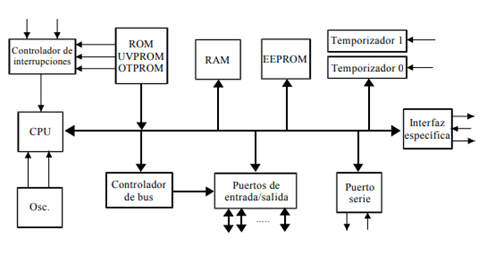
\includegraphics[scale = 0.95]{Imagenes/CAP2_elementos_microcontrolador.png}
    \caption{Elementos de un microcontrolador}{Fuente: Adaptado de~\cite{microcontroladores}}
\end{figure}

\subsection{Uso de Arduino y ESP32}

Arduino es una placa de desarrollo de hardware libre, que puede ser utilizada tanto por aficionados como por fabricantes para diseñar y construir dispositivos que interactúen con el mundo real, a través de una gran cantidad de sensores y otros elementos electrónicos que están disponibles en el mercado. Aunque utilizamos el término Arduino para referirnos a un tipo específico de placa de desarrollo, también se usa para hablar de la empresa que fabrica estas placas o para describir a la comunidad en torno a las diferentes placas compatibles \cite{pena}.

\textbf{Clasificación Dse Pines}

\subsubsection{Pines analógicos}
Los pines analógicos pueden leer un amplio rango de valores, por lo que son útiles para realizar un control más detallado de las lecturas obtenidas. En general se encuentran 6 pines y mediante estos pines es posible obtener datos de sensores en forma de variaciones continuas de un voltaje. 

\subsubsection{Pines digitales}
Los pines digitales son capaces de leer y escribir un solo estado, es decir, encendido o apagado. En la mayoría de las placas Arduino hay 14 pines \cite{pena}.

\begin{figure}[H]
     \centering
     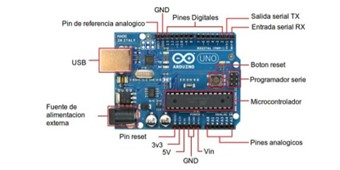
\includegraphics[scale = 0.97]{Imagenes/ardr3.jpg}
     \caption{Arduino UNO R3}{Fuente: Adaptado de ~\cite{mecafenix}}
\end{figure}

\textbf{ESP32}

Plataforma de  hardware  abierto, basada   en   un   sistema  en  chip  (SoC,  del  inglés  System on  a  Chip) con hardware específico para comunicaciones inalámbricas, entre otros recursos. Este  permite  el  desarrollo  de  aplicaciones  en  diferentes  lenguajes  de  programación,  frameworks, bibliotecas  y  recursos  diversos.

El  SoC  ESP32  de  Espressif  Systems  es  la  evolución  del  ESP8266,  diseñado  para  superar  a  su  antecesor  en  capacidad  de  procesamiento  y  conectividad;  integra  un  potente  microcontrolador  con  arquitectu-ra de 32 bits, conectividad wifi y Bluetooth. El  sistema  en  el  módulo  (SoM,  del  inglés  System  on  Module)  ESP-32S  fabricado  por  Ai-Thinker  integra  en  un  módulo  el  SoC  ESP32, memoria FLASH, cristal oscilador y antena wifi en PCB.

\begin{figure}[htb]
    \centering
    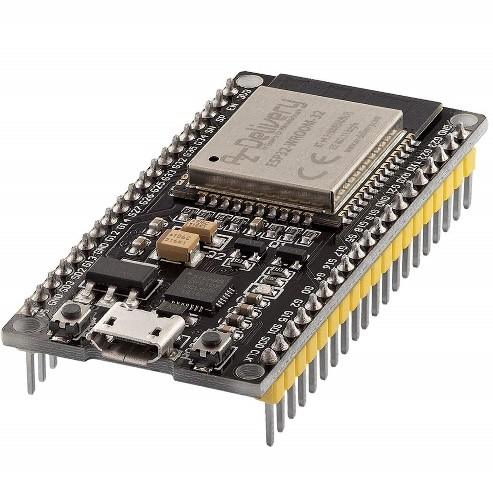
\includegraphics[scale = 0.50]{Imagenes/esp32cam.jpg}
    \caption{ESP32}{Fuente: Adaptado de ~\cite{delivery}}
\end{figure}

Se destaca el módulo ESP32-CAM, que incluye una cámara OV2640 y varios GPIO para conectar periféricos usando un ESP32. El módulo también cuenta con una ranura para tarjeta microSD, que permite almacenar imágenes tomadas de la cámara o almacenar archivos y viene con el módulo de cámara de 2MP. Las funcionalidades de este módulo y su capacidad de realizar diversas tareas lo han convertido en un componente eficaz para la seguridad. Este módulo se puede utilizar en videovigilancia para transmitir imágenes o funcionar como sensores en un sistema de visión \cite{salvador}.

\begin{figure}[htb]
    \centering
    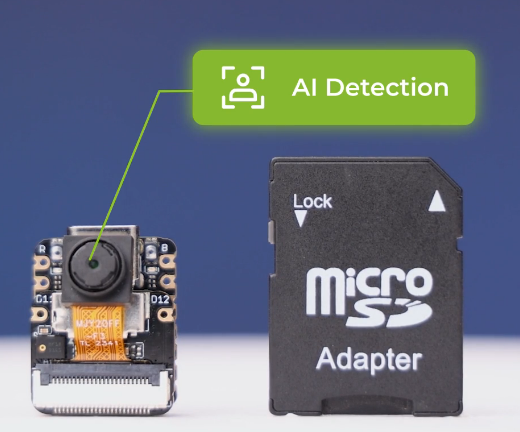
\includegraphics[scale = 0.50]{Imagenes/xiao esp32cam.png}
    \caption{XIAO ESP32 CAM}{Fuente: Adaptado de~\cite{foto_xiao}}
\end{figure}

\subsection{Sistemas de clasificación automática}
Machine Learning es un área de la inteligencia artificial que engloba un conjunto de técnicas que hacen posible el aprendizaje automático a través del entrenamiento con grandes volúmenes de datos. Hoy en día, existen diferentes modelos que utilizan esta técnica y consiguen una precisión incluso superior a la de los humanos en las mismas tareas, por ejemplo, en el reconocimiento de objetos en una imagen. La construcción de modelos de Machine Learning requiere adaptaciones propias debido a la naturaleza de los datos o a la problemática a la que se aplica. Así, surge la necesidad de investigar las diferentes técnicas que permitan obtener resultados precisos y confiables en un tiempo razonable \cite{russo}.

Dentro de esta clasificación, podemos además encontrar un gran número de algoritmos específicos con diferentes características para el tratamiento de los datos. Entre los más relevantes encontramos:

\begin{itemize}
    \item \textbf{Deep Learning}: consiste en la utilización de algoritmos para hacer representaciones abstractas de la información y facilitar el aprendizaje automático.
    \item \textbf{Active Learning}: es un caso especial de aprendizaje semi-supervisado donde el algoritmo de aprendizaje puede interactuar con un usuario u otra fuente de información para obtener los resultados deseados.
    \item \textbf{Support Vector Machines}: busca la maximización de la distancia entre la recta o el plano y las muestras que se encuentran a un lado u otro. En el caso de que las muestras no sean linealmente separables, se utiliza una transformación llamada kernel.

    La teoría de las Máquinas de Soporte Vectorial (SVM, por su nombre en inglés, Support Vector Machines) es una nueva técnica de clasificación y ha tomado mucha atención en años recientes. La teoría de la SVM está basada en la idea de minimización de riesgo estructural (SRM). En muchas aplicaciones, las SVM han mostrado tener un gran desempeño más que las máquinas de aprendizaje tradicional como las redes neuronales y han sido introducidas como herramientas poderosas para resolver problemas de clasificación.
\end{itemize}

\begin{figure}[htb]
	\centering
	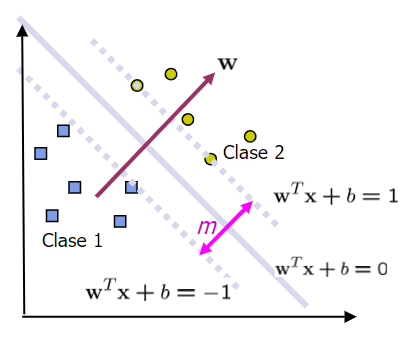
\includegraphics[scale  = 0.70]{Imagenes/maxim.png}
	\caption{Margen m maximizado}{Fuente: Adaptado de ~\cite{betancourt}}
\end{figure}

Una Máquina de Soporte Vectorial (SVM) aprende la superficie de decisión de dos clases distintas de los puntos de entrada. Como un clasificador de una sola clase, la descripción dada por los datos de los vectores de soporte es capaz de formar una frontera de decisión alrededor del dominio de los datos de aprendizaje con muy poco o ningún conocimiento de los datos fuera de esta frontera \cite{betancourt}.
\subsection{Aplicaciones de IoT}

\textbf{Comunicación y monitoreo}

El IoT tiene una amplia gama de aplicaciones en diversos sectores como se muestra en la ilustración No. 1. En el ámbito de la salud, el IoT se utiliza para monitorear pacientes y proporcionar atención médica remota. En el transporte, el IoT permite la gestión de flotas de vehículos y el seguimiento en tiempo real de la ubicación de mercancías. En la agricultura, el IoT se aplica para el monitoreo y control de cultivos, optimizando el riego y la fertilización. Además, el IoT ha encontrado aplicaciones en ciudades inteligentes, hogares inteligentes, industria manufacturera, entre otros campos.

\begin{figure}[htb]
	\centering
	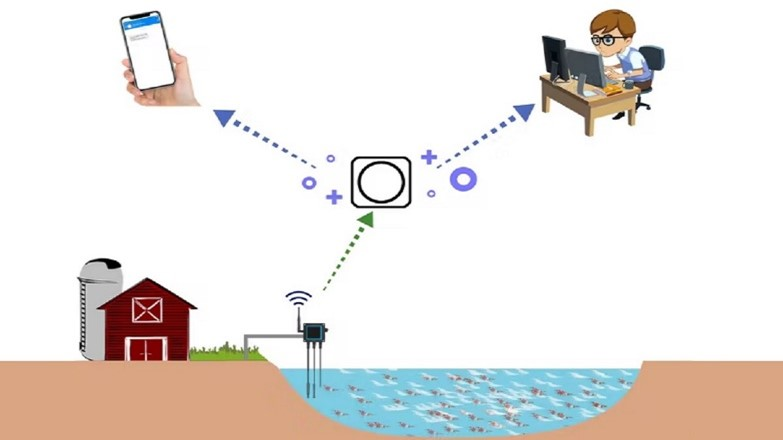
\includegraphics[scale  = 0.80]{Imagenes/iot.jpg}
	\caption{Sistema de monitoreo de acuicultura - Tecnologia Humanizada}{Fuente: Adaptado de~\cite{udin}}
\end{figure}

Sin embargo, la implementación exitosa de IoT en la recolección de residuos sólidos requiere de un enfoque integral que abarque aspectos técnicos, operativos y de privacidad de los datos. En la literatura científica existen algunos trabajos con propósitos similares que utilizan metodologías, arquitecturas y equipos diferentes, a continuación, se detallan.

Tarandeep Singh, en su trabajo denominado \textit{IOT based Smart Waste Management Framework (Singh)}, proporciona una solución para mejorar la gestión de residuos sólidos mediante la monitorización remota de los parámetros de los contenedores de basura y la optimización de las rutas de recolección. La metodología utiliza la tecnología X-bee y GSM para monitorear de forma remota los parámetros de los contenedores, como el llenado del contenedor, la temperatura, la humedad y el volumen de CO2 dentro del contenedor. Los datos recopilados se transmiten a una estación base que los envía a una estación de control para su análisis y optimización de rutas de recolección de basura. Las conclusiones del estudio sugieren que el uso de tecnología IoT en la gestión de residuos sólidos puede ser una solución efectiva y rentable para mejorar la eficiencia de la recolección de basura y reducir los costos operativos y las emisiones de gases de efecto invernadero.

Mientras tanto, Raúl Hernández y su equipo analizan la gestión y el proceso de recolección de residuos sólidos urbanos (RSU) en el municipio de Nezahualcóyotl, Estado de México, donde identifican las principales características de la gestión y recolección de RSU en el municipio y aplican la idea de la Ciudad Inteligente (CI) para mejorar el servicio de recolección de basura \cite{sinaluisa}.

La aplicación del Internet de las Cosas (IoT) en sistemas de clasificación de basura es una tendencia innovadora para mejorar la gestión de residuos. 

Sistemas de clasificación automática basados en cámaras y sensores ópticos conectados a la red IoT pueden identificar diferentes tipos de residuos (plásticos, metales, vidrio, etc.). Esto mejora la eficiencia del reciclaje al separar automáticamente los residuos según su tipo.

\begin{figure}[htb]
	\centering
	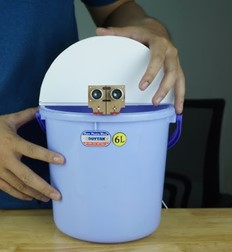
\includegraphics[scale  = 0.90]{Imagenes/iot_contenedor.jpg}
	\caption{IoT - contenedor de basura inteligente}{Fuente: Adaptado de~\cite{logic}}

\end{figure}

Las plataformas IoT permiten a los gestores de residuos monitorear remotamente el estado de los contenedores y otros equipos en tiempo real, lo que mejora la eficiencia operativa y reduce el tiempo de inactividad.
\subsection{Campo de aplicación}

\textbf{Contenedores de Basura Inteligentes}

Los contenedores de basura inteligentes encuentran aplicaciones en varios sectores:

\subsubsection{Entornos Urbanos}
En ciudades y municipios, los contenedores de basura inteligentes están ayudando a gestionar grandes volúmenes de residuos de manera eficiente. Son particularmente útiles en áreas de mucho tráfico, ya que reducen la carga de trabajo de los equipos de recolección de residuos \cite{buying}.

El Internet de las Cosas está teniendo un impacto tanto en la industria como en la vida cotidiana de las personas. Actualmente existen contenedores de basura inteligentes, que han funcionado exitosamente en ciudades como Sevilla. A través del proyecto europeo LIFE EWAS, se ha implementado una solución de TICS que permite monitorizar el volumen de llenado de los contenedores. Se implementan sensores con sistemas de medidas volumétricas basados en parámetros como la distancia, es decir, el trecho entre el nivel de residuos y el sensor. Esta información permite conocer la capacidad de un contenedor. Al dotar de inteligencia al contenedor, se puede entregar información a un gestor de servicios, optimizando así la recolección de los residuos \cite{quimbita}.

\begin{figure}[htb]
	\centering
	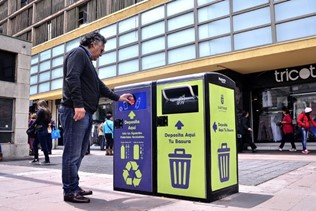
\includegraphics[scale  = 0.90]{Imagenes/basurero int.jpg}
	\caption{Basurero inteligente}{Fuente: Adaptado de~\cite{chile}}

\end{figure}

\subsubsection{Espacios Comerciales}
En entornos comerciales, como centros comerciales y aeropuertos, los contenedores inteligentes mejoran la gestión de residuos, asegurando que se vacíen rápidamente y reduciendo las molestias del desbordamiento de basura \cite{buying}.

\subsubsection{Industria Hotelera}
Los hoteles y restaurantes están utilizando contenedores inteligentes para mantener la limpieza y la higiene, brindando una mejor experiencia a los huéspedes \cite{buying}. Los botes de basura inteligentes pueden mejorar la experiencia del cliente proporcionando una gestión automática y sin contacto, aumentando la comodidad y reduciendo la necesidad de mantenimiento frecuente. Pueden notificar cuando están llenos, asegurando que el personal de limpieza los vacíe de manera oportuna, lo cual es una buena manera de asegurar que los clientes no se disgusten y se sientan bien atendidos.

\subsubsection{Instalaciones Sanitarias}
En entornos sanitarios, donde la higiene es primordial, los contenedores de basura inteligentes desempeñan un papel crucial en la gestión eficiente de residuos y el control de infecciones \cite{buying}.

\subsubsection{Instituciones Educativas}
Las escuelas y universidades están utilizando contenedores inteligentes para enseñar a los estudiantes sobre la eliminación responsable de residuos y, al mismo tiempo, mantener limpios sus campus. Este es uno de los campos de aplicación que motivan este proyecto, ya que son situaciones comunes en las instituciones educativas en el día a día.

\subsection{Futuro del tema de investigación}

\textbf{Acceso biométrico:} Se pueden incorporar funciones biométricas como el reconocimiento de huellas dactilares en los contenedores inteligentes para evitar el uso no autorizado y mejorar la seguridad.

\textbf{Conectividad mejorada:} Los contenedores inteligentes pueden convertirse en parte de redes más grandes de ciudades inteligentes, permitiendo la comunicación en tiempo real con otros sistemas municipales, como la gestión del tráfico.

\section{Proyectos similares}

Existen proyectos similares que se han realizado anteriormente:

\subsection{Diseño de un Contenedor Municipal Automático}
“DISEÑO DE UN CONTENEDOR MUNICIPAL AUTOMÁTICO MEDIANTE RED DE SENSORES CON MONITOREO INALÁMBRICO PARA LA MEJORA DEL PROCESO DE SELECCIÓN DE RESIDUOS SÓLIDOS, CALLAO 2022”. Este trabajo de investigación tiene como fin plantear una solución a una realidad que afecta a la sociedad actual, específicamente en el entorno urbano, donde la población citadina crece año tras año debido al centralismo. Este crecimiento poblacional conlleva un aumento en la producción de residuos de diversas categorías, entre ellos, los residuos sólidos. 

Como objetivo general, tiene diseñar un contenedor municipal automático mediante red de sensores y monitoreo inalámbrico, capaz de mejorar el proceso de selección de residuos sólidos. El sistema utiliza sensores y un microcontrolador para distinguir entre diferentes tipos de desechos, como plástico, vidrio, cartón y papel. El resultado final de este proyecto es un prototipo de un contenedor de residuos sólidos inteligente, que tiene instalado un módulo GPS para controlar la ubicación y un sensor ultrasónico que mide el nivel de llenado. En la Figura 90 se muestra el diseño del dispositivo que será ubicado dentro de un contenedor de residuos sólidos. Este dispositivo se compone de un sensor ultrasónico, un módulo GPS, un módulo ESP32 con su batería recargable, un transceptor LoRa RFM95 con una antena helicoidal y un panel solar para cargar las baterías de litio \cite{manrique}.

\subsection{Sistema de Clasificación Inteligente de Residuos}
“INTELLIGENT WASTE SORTING SYSTEM: LEVERAGING ARDUINO FOR AUTOMATED TRASH IDENTIFICATION AND CATEGORIZATION”. En este trabajo de investigación, se utiliza un conjunto de datos personalizado, una colección completa de imágenes de categorías de desechos divididas en siete clases, con modelos de detección de objetos como YOLO para automatizar la detección de basura y la clasificación precisa, mejorando así la precisión en la clasificación de desechos. El objetivo principal es aprovechar los atributos distintivos de los modelos YOLO combinados con Arduino para desarrollar un sistema de clasificación de basura más eficaz. Los procesos tradicionales de gestión de basura son laboriosos, lo que los hace lentos, costosos y propensos a errores humanos. Para superar estas deficiencias, se propone un modelo basado en el aprendizaje profundo que pueda detectar y clasificar rápidamente varios tipos de desechos en tiempo real. YOLO, un algoritmo de detección de objetos de última generación, sirve como columna vertebral de este modelo, asegurando una identificación rápida y precisa de los desechos. La integración de un microcontrolador Arduino agrega una dimensión práctica e interactiva, facilitando la comunicación entre el modelo de aprendizaje profundo y el mundo físico, permitiendo que el sistema active acciones como la clasificación, el reciclaje o la alerta a las autoridades \cite{ali}.

\subsection{Contenedor de Reciclaje Automatizado de Bajo Costo}
“A LOW-COST AUTOMATED SORTING RECYCLE BIN POWERED BY ARDUINO MICROCONTROLLER”. Este artículo presenta el desarrollo de un contenedor de reciclaje de bajo costo que clasifica automáticamente diferentes tipos de desechos reciclables utilizando un microcontrolador Arduino. Los objetivos de este trabajo son construir un prototipo de contenedor de reciclaje con un mecanismo de detección que pueda clasificar los desechos reciclables (como metal, papel y plástico) y asignar automáticamente los desechos a particiones específicas del contenedor según sus tipos. Este artículo también presenta el análisis de sensibilidad del prototipo de contenedor de reciclaje para clasificar los desechos correctamente. La construcción del prototipo se divide en dos partes: i) detección y ii) mecánica. La parte de detección identifica el tipo de material de desecho, utilizando un sensor de proximidad inductivo para detectar metales y un diodo emisor de luz (LED) junto con una resistencia dependiente de la luz (LDR) para papel y plástico. La parte mecánica incorpora un servomotor junto con el microcontrolador para clasificar el tipo de desecho. Los resultados muestran que el prototipo es capaz de clasificar los residuos con éxito, especialmente los plásticos, aunque se necesita mejorar la sensibilidad a los residuos de papel y metal para lograr una segregación eficaz \cite{hassan}.

\section{Tecnologías De Desarrollo}
\subsection{Arduino UNO R3}

Esta tarjeta se encarga de recibir y almacenar el orden de cada señal entregada ~\cite{buitrago}. 

Es el microcontrolador principal que controla todas las funciones básicas del sistema, como leer datos de los sensores (nivel de llenado, detección de movimiento) y activar los actuadores (abrir/cerrar la tapa del cubo). También es el que recibe las señales de los sensores y ejecuta las acciones correspondientes, como encender un buzzer o enviar alertas.


\begin{figure}[htb]
	\centering
	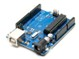
\includegraphics[scale  = 0.50]{Imagenes/uno3.jpg}
	\caption{ARDUINO UNO R3 }{Fuente: Adaptado de~\cite{mecafenix}}

\end{figure}

\subsection{IDE Arduino}

El entorno de programaciónde la  placa  de  Arduino  se denomina Integrated  Development  Environment (IDE)el cual  permite  llevar  a  cabo  la  escritura  de  las  sentencias para el funcionamiento de los elementos físicos de la placa de Arduino. Este   software   tiene   por   si   solo   un   conjunto   de herramientas que permite,  editar  el  código,  compilar  y depurar todo a través de una interfaz gráfica, así mismo, nos    da    la    oportunidad    de    interactuar    con    el microcontrolador almacenando los programas  realizados en  su  memoria  interna  para  poner  en  marcha  todo  el hardware. El lenguaje que utiliza el IDE de Arduino está basado en C/C++ de una manera más simplificada, ofreciendo la oportunidad de cargar librerías que sean necesarias para el buen funcionamiento de nuestros proyectos ~\cite{perez}.

\begin{figure}[htb]
	\centering
	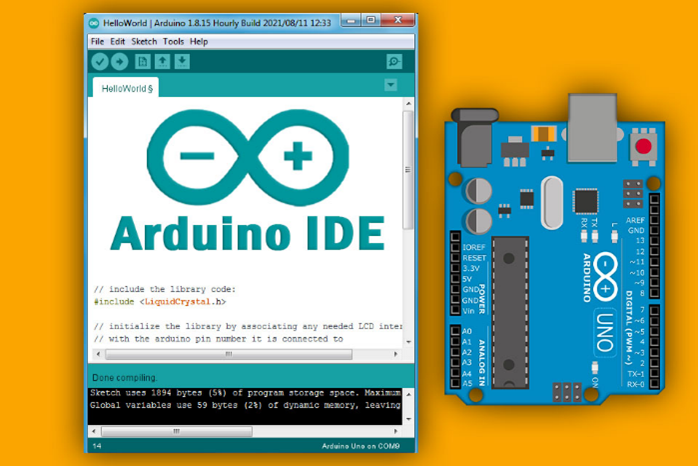
\includegraphics[scale  = 0.80]{Imagenes/ide.png}
	\caption{IDE Arduino}{Fuente: Adaptado de~\cite{perez}}

\end{figure}

\subsection{Micropython}

MicroPython es una reimplementación del lenguaje de programación Python que apunta a microcontroladores y sistemas integrados.

Los microcontroladores son computadoras compactadas en un solo chip muy pequeño. Los sistemas integrados son computadoras que funcionan dentro de un sistema mecánico o eléctrico más grande~\cite{tollervey}.

Los sistemas integrados a menudo utilizan microcontroladores.

\begin{figure}[H]
	\centering
	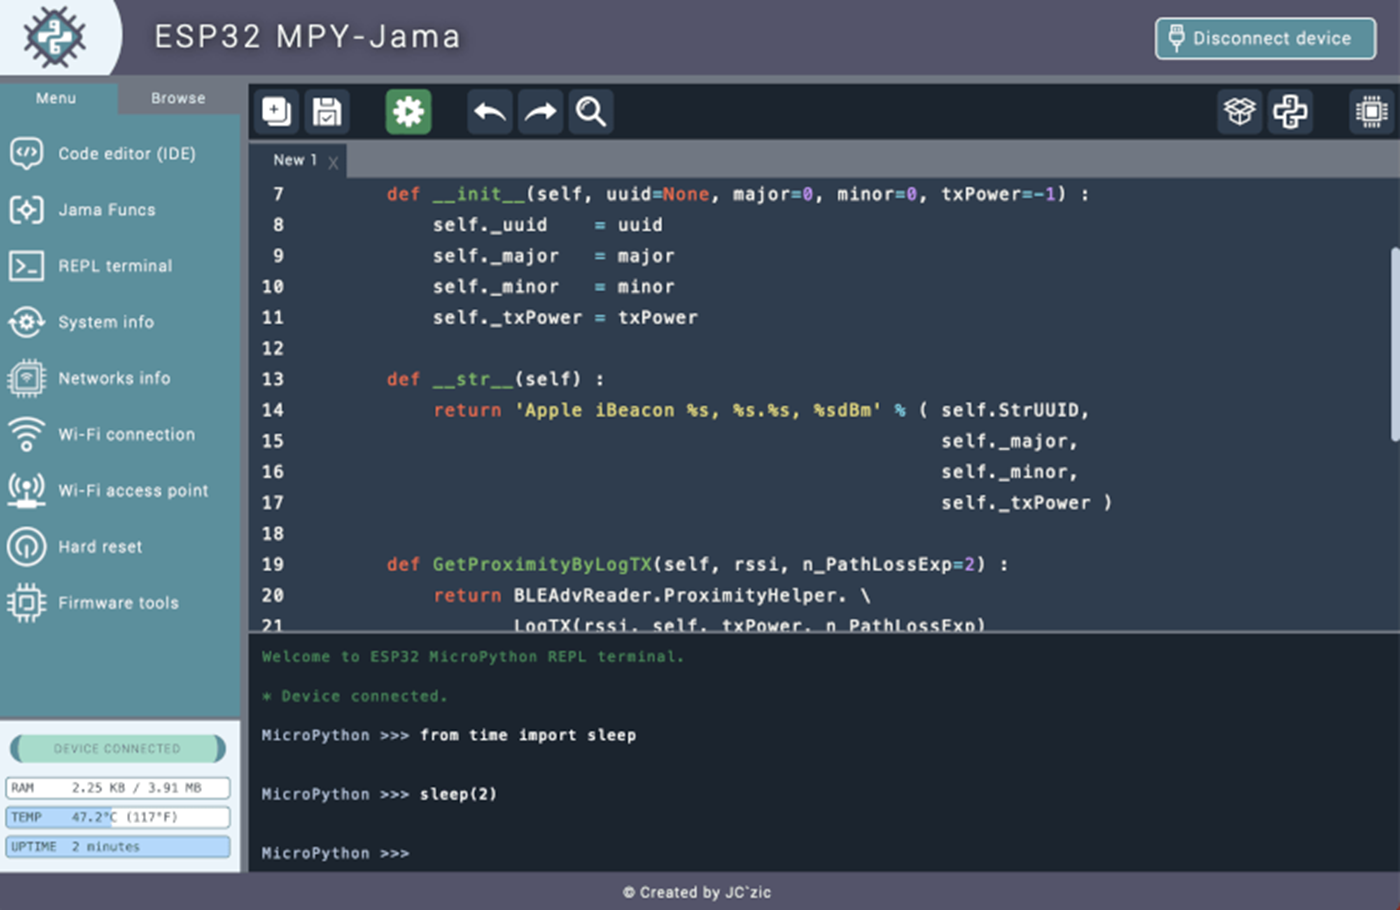
\includegraphics[scale  = 0.60]{Imagenes/mycro.png}
	\caption{Interfaz de MicroPython}{Fuente: Adaptado de~\cite{mpy}}
\end{figure}


\subsection{CNN}

Una red neuronal convolucional es un tipo de red neuronal artificial donde las neuronas artificiales, corresponden a campos receptivos de una manera muy similar a las neuronas en la corteza visual primaria (V1) de un cerebro biológico. Este tipo de red es una variación de un perceptron multicapa, sin embargo, debido a que su aplicación es realizada en matrices bidimensionales, son muy efectivas para tareas de visión artificial, como en la clasificación y segmentación de imágenes, entre otras aplicaciones~\cite{red_neuronal}.

\begin{figure}[htb]
	\centering
	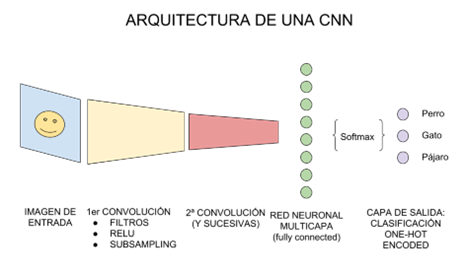
\includegraphics[scale  = 0.80]{Imagenes/cnn.png}
	\caption{Arquitectura de una red CNN}{Fuente: Adaptado de~\cite{red_neuronal}}

\end{figure}

\subsection{Visión Artificial}

Es una disciplina científica que incluye métodos para adquirir, procesar, analizar y comprender las imágenes del mundo real con el fin de producir información numérica o simbólica para que puedan ser tratados por un ordenador. Tal y como los seres humanos usamos nuestros ojos y cerebros para comprender el mundo que nos rodea, la visión informática trata de producir el mismo efecto para que los ordenadores puedan percibir y comprender una imagen o secuencia de imágenes y actuar según convenga en una determinada situación. Esta comprensión se consigue gracias a distintos campos como la geometría, la estadística, la física y otras disciplinas. La adquisición de los datos se consigue por varios medios como secuencias de imágenes, vistas desde varias cámaras de video o datos multidimensionales desde un escáner médico~\cite{vision_artificial}.

\subsection{Open CV}

\textbf{OpenCV} es una biblioteca libre de visión artificial originalmente desarrollada por Intel. OpenCV significa Open Computer Vision (Visión Artificial Abierta). OpenCV ofrece soporte para varios sistemas operativos y varias arquitecturas de hardware, pero también ofrece el código fuente para que cualquier desarrollador lo compile en cualquier sistemas operativo y arquitectura particular~\cite{opencv}. 

OpenCV y ESP32 se pueden utilizar juntos para crear sistemas de visión integrados, en los que se pueden ejecutar tareas de visión por computadora simples en un microcontrolador ESP32.

\begin{figure}[htb]
	\centering
	
\includegraphics[scale  = 0.80]{Imagenes/opencv.png}
	\caption{Logo de OpenCV}{Fuente: Adaptado de~\cite{opencv}}

\end{figure}

\subsubsection{Numpy}

NumPy es una biblioteca para el lenguaje de programación Python, que agrega soporte para matrices y arreglos multidimensionales grandes, junto con una gran colección de funciones matemáticas de alto nivel para operar en estos arreglos~\cite{numpy}.

\begin{figure}[htb]
	\centering
	
\includegraphics[scale  = 0.80]{Imagenes/numpy.png}
	\caption{Logo de Numpy}{Fuente: Adaptado de~\cite{numpy}}
\end{figure}

\subsection{XIAO ESP32 CAM}
El ESP32-CAM es un módulo de cámara muy pequeño y económico que cuenta con el chip ESP32-S. Además de la cámara OV2640 y varios GPIO para conectar periféricos, también cuenta con una ranura para tarjeta microSD que puede ser útil para almacenar imágenes tomadas con la cámara o para almacenar archivos para servir a los clientes 

\begin{figure}[htb]
	\centering
	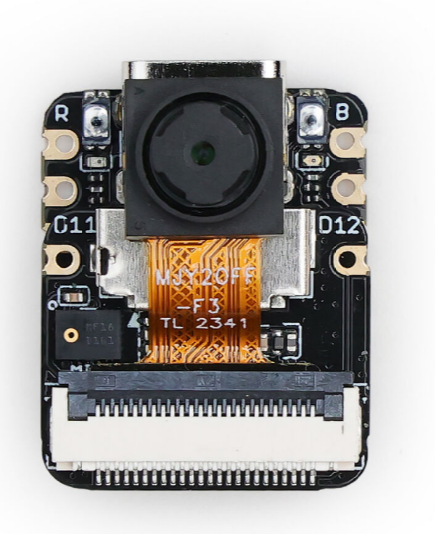
\includegraphics[scale  = 0.70]{Imagenes/xiao.png}
	\caption{XIAO ESP32 CAM}{Fuente: Adaptado de~\cite{foto_xiao}}
\end{figure}

A continuación, se presenta el DataSheet encontrado.

\begin{table}[H]
    \centering
    \begin{tabularx}{\textwidth}{|l|X|} % Usar X para columnas que se expanden
        \hline
        \textbf{Ítem} & \textbf{Descripción} \\ 
        \hline
        \textbf{Procesador} & ESP32-S3R8, Xtensa LX7 de doble núcleo, 32 bits, hasta 240 MHz \\ 
        \hline
        \textbf{Inalámbrico} & Subsistema Wi-Fi completo de 2.4GHz, BLE: Bluetooth 5.0, Bluetooth mesh \\ 
        \hline
        \textbf{Sensores Integrados} & Sensor de cámara OV2640 (1600*1200), Micrófono digital \\ 
        \hline
        \textbf{Memoria} & 8M PSRAM y 8MB Flash en chip, Ranura para tarjeta SD (hasta 32GB FAT) \\ 
        \hline
        \textbf{Interfaz} & 1x UART, 1x IIC, 1x IIS, 1x SPI, 11x GPIOs (PWM), 9x ADC, 1x LED de usuario, 1x LED de carga \\ 
        & 1x conector B2B (2 GPIOs adicionales), 1x botón de reinicio, 1x botón de arranque \\ 
        \hline
        \textbf{Dimensiones} & 21 x 17.8 x 15 mm (con placa de expansión) \\ 
        \hline
        \textbf{Alimentación} & Voltaje de entrada (Type-C): 5V, Voltaje de entrada (BAT): 4.2V \\ 
        & Voltaje de operación (Type-C): 5V@38.3mA, Voltaje de operación (BAT): 3.8V@43.2mA (con expansión) \\ 
        \hline
        \textbf{Modelo de Bajo Consumo} & Sueño de módem: ~44mA, Sueño ligero: ~5mA, Sueño profundo: ~3mA \\ 
        \hline
        \textbf{Consumo de Potencia (Wi-Fi)} & Modelo activo: ~110 mA (con expansión) \\ 
        \hline
        \textbf{Consumo de Potencia (BLE)} & Modelo activo: ~102 mA (con expansión) \\ 
        \hline
        \textbf{Temperatura de Funcionamiento} & -40°C ~ 65°C \\ 
        \hline
    \end{tabularx}
    \caption{DataSheet de la XIAO ESP32 CAM}{Fuente: ~\cite{xiaotabla}}
\end{table}

\subsection{Sensor ultrasónico (HC-SR04)}

Este sensor mide la distancia entre el sensor y el nivel de basura dentro del cubo. Con esta información, se puede calcular el porcentaje de llenado. Funciona enviando pulsos ultrasónicos y midiendo el tiempo que tarda en regresar el eco, lo que indica la distancia al objeto más cercano (en este caso, la basura).

\begin{figure}[htb]
	\centering
	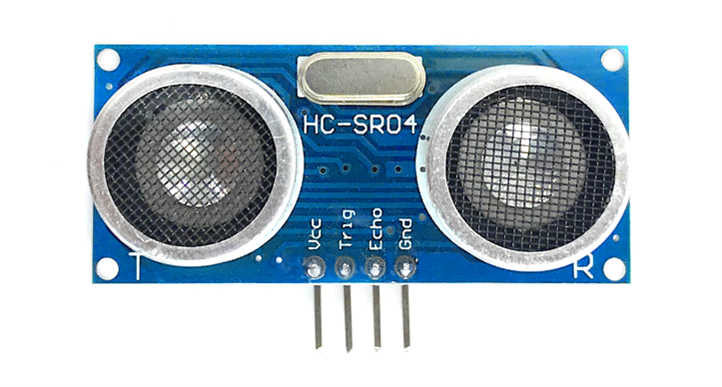
\includegraphics[scale  = 0.50]{Imagenes/ultra.png}
	\caption{Sensor ultrasónico HC-SR04}{Fuente: Adaptado de~\cite{ultrasonc}}

\end{figure}

\begin{table}[H]
    \centering
    \begin{tabularx}{\textwidth}{|l|X|} % Usar X para columnas que se expanden
        \hline
        \textbf{Especificación} & \textbf{Descripción} \\ 
        \hline
        \textbf{Voltaje de funcionamiento} & DC 5V \\ 
        \hline
        \textbf{Corriente de funcionamiento} & 15mA \\ 
        \hline
        \textbf{Frecuencia de funcionamiento} & 40kHz \\ 
        \hline
        \textbf{Alcance máximo} & 4 m \\ 
        \hline
        \textbf{Alcance mínimo} & 2 cm \\ 
        \hline
        \textbf{Precisión de medición} & 3 mm \\ 
        \hline
        \textbf{Ángulo de medición} & 15 grados \\ 
        \hline
        \textbf{Señal de entrada del disparador} & Pulso TTL de 10 µs \\ 
        \hline
        \textbf{Dimensiones} & 45 x 20 x 15 mm \\ 
        \hline
    \end{tabularx}
    \caption{Especificaciones del HC-SR04}{Fuente: Adaptado de~\cite{ultrasonc}}
    \label{tab:especificaciones_hc_sr04}
\end{table}

\subsection{Cables jumper, resistencias, protoboard}

Estos componentes se utilizan para conectar todos los sensores, microcontroladores y actuadores de manera temporal o durante la fase de pruebas. Los cables jumper permiten hacer conexiones rápidas entre pines, y la protoboard facilita las conexiones sin necesidad de soldar.

\begin{figure}[htb]
	\centering
	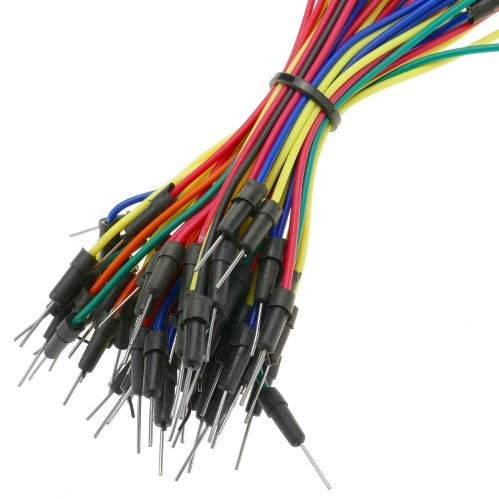
\includegraphics[scale  = 0.50]{Imagenes/jumper.jpg}
	\caption{Jumpers}{Fuente: Propia}
\end{figure}

\begin{figure}[htb]
	\centering
	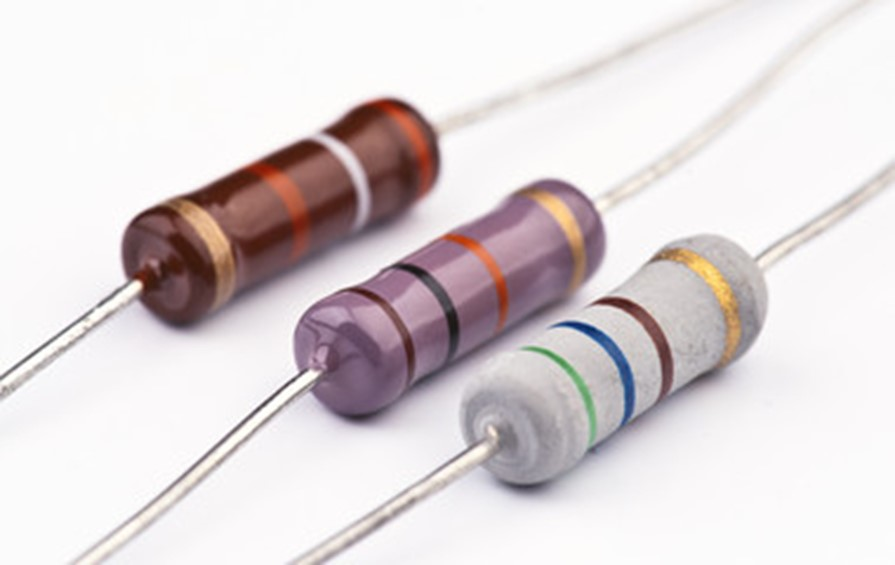
\includegraphics[scale  = 0.50]{Imagenes/resistores.jpg}
	\caption{Resistores}{Fuente: Propia}
\end{figure}

\begin{figure}[htb]
	\centering
	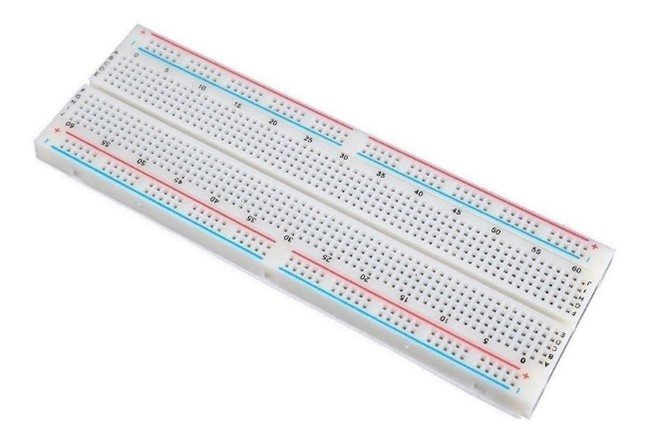
\includegraphics[scale  = 0.50]{Imagenes/bread.jpg}
	\caption{ProtoBoard}{Fuente: Propia}
\end{figure}

\subsection{Servomotor (SG90)}
El SG90 es un servo miniatura de gran calidad y diminutas dimensiones, además es bastante económico. Funciona con la mayoría de las tarjetas electrónicas de control con microcontroladores y además con la mayoría de los sistemas de radio control comerciales. Funciona especialmente bien en aeronaves dadas sus características de torque, tamaño y peso.

El servo SG90 tiene un conector universal tipo “S” que encaja perfectamente en la mayoría de los receptores de radio control incluyendo los Futaba, JR, GWS, Cirrus, Hitec y otros. Los cables en el conector están distribuidos de la siguiente forma: Rojo = Alimentación (+), Cafe = Alimentación (-) o tierra, Naranjo = Señal PWM.

Este tipo de servo es ideal para las primeras experiencias de aprendizaje y prácticas con servos, ya que sus requerimientos de energía son bastante bajos y se permite alimentarlo con la misma fuente de alimentación que el circuito de control. Por ejemplo, si se conecta a una tarjeta arduino, se puede alimentar durante las pruebas desde el puerto USB de la PC sin mayor problema~\cite{servo_motor}.

\begin{figure}[H]
	\centering
	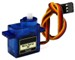
\includegraphics[scale  = 0.50]{Imagenes/micro.jpg}
	\caption{Mini Sevo motor}{Fuente: Adaptado de~\cite{servo_motor}}
\end{figure}

A continuación, se muestra el DataSheet encontrado:

\begin{table}[H]
    \centering
    \begin{tabularx}{\textwidth}{|l|X|} % Usar X para columnas que se expanden
        \hline
        \textbf{Especificación} & \textbf{Descripción} \\ 
        \hline
        \textbf{Dimensiones} & 22mm x 11,5mm x 27mm \\ 
        \hline
        \textbf{Peso} & 9 gramos \\ 
        \hline
        \textbf{Peso con cable y conector} & 10.6 gramos \\ 
        \hline
        \textbf{Torque a 4.8 volts} & 1.2 kg/cm \\ 
        \hline
        \textbf{Voltaje de operación} & 4.0 a 7.2 volts \\ 
        \hline
        \textbf{Velocidad de giro a 4.8 volts} & 120 ms / 60 º \\ 
        \hline
        \textbf{Conector} & Universal para la mayoría de los receptores de radio control \\ 
        \hline
        \textbf{Compatibilidad} & Compatible con tarjetas como Arduino y microcontroladores que funcionan a 5 volts. \\ 
        \hline
    \end{tabularx}
    \caption{Especificaciones del SG90}{Fuente: Adaptado de~\cite{servo_motor}}
    \label{tab:especificaciones_sg90}
\end{table}

%CAPITULO 3 
\chapter{Capítulo 3: Propuesta del Proyecto}
\section{Metodo-Experimentación}
\subsection{Tipo y alcance de la investigación}
La investigación es de tipo experimental con el diseño de un prototipo funcional, que emplea tecnologías de reconocimiento de imágenes y sensores ultrasónicos para clasificar de manera automática los residuos. Esto permite validar la hipótesis mediante pruebas en condiciones reales, evaluando la efectividad del sistema en clasificar diferentes tipos de materiales y contribuyendo a la reducción de residuos no clasificados correctamente.

La elección de un enfoque experimental obedece a la necesidad de observar y medir la precisión del sistema en un entorno controlado antes de una posible implementación a gran escala. Este tipo de investigación también permite hacer ajustes y mejoras al prototipo en función de los resultados obtenidos durante las pruebas.


El alcance del proyecto es de prueba de concepto, es decir, se busca construir un prototipo funcional que demuestre la viabilidad y eficacia de una solución automatizada para la clasificación de residuos. Al limitar el alcance a una prueba de concepto, se facilita el desarrollo inicial, y se enfoca en comprobar si la tecnología y el diseño propuestos cumplen con los objetivos de clasificación eficiente y mejora en la gestión de residuos.

Este prototipo servirá como base para evaluaciones futuras, pudiendo ser optimizado para aplicaciones más amplias en el campus o en otros contextos similares. Al finalizar el proyecto, se espera contar con datos que validen la hipótesis y ofrezcan una visión clara de los beneficios potenciales de la tecnología aplicada.
\subsection{Observación}
\input{3.1 Metodo-Experimentacion/3.1.1 Observación.tex}
\subsection{Planteamiento de Hipótesis}
Con la observación presentada anteriormente, nos hacemos la siguiente pregunta:
\textbf{¿Cómo eliminamos la mezcla de desechos que dificulta la separación para reciclables?}

Nuestra hipótesis radica en la implementación de un sistema automatizado de clasificación de residuos que utilice tecnología de reconocimiento de imágenes (ESP32 CAM) aumentará la tasa de reciclaje en el centro regional de Veraguas al facilitar la separación de materiales reciclables y sensibilizar a la comunidad universitaria sobre la importancia del reciclaje.
\subsection{Experimentación}
\input{3.1 Metodo-Experimentacion/3.1.3 Experimentación.tex}
\subsection{Análisis de Datos}
Con el prototipo desarrollado esperamos obtener los siguientes datos:

\begin{enumerate}
    \item \textbf{Cantidad Total de Residuos:} Registrar el volumen total de residuos que se depositan en el basurero inteligente.
    \item \textbf{Cantidad de Residuos Clasificados Correctamente:} Contar cuántos residuos fueron identificados y clasificados correctamente por el sistema en comparación con los incorrectamente clasificados.
\end{enumerate}

\textbf{Generar gráficos para la precisión del algoritmo de clasificación}

Esta recolección de data nos permite los siguientes puntos:

\begin{enumerate}
    \item \textbf{Visualizar de forma clara los datos}
    \begin{enumerate}
        \item \textbf{La Comprensión}: Los gráficos transforman datos numéricos en visualizaciones fáciles de interpretar, lo que permite comprender rápidamente el rendimiento del algoritmo sin necesidad de analizar tablas complejas.
        \item \textbf{Identificar tendencias}: A través de gráficos de líneas podremos observar cómo la precisión ha cambiado a lo largo del tiempo, lo que puede indicar si el sistema está mejorando con el uso.
    \end{enumerate}
    
    \item \textbf{Comparar}
    \begin{enumerate}
        \item \textbf{Comparación entre categorías}: Con gráficos de barras, podemos comparar la precisión entre diferentes categorías de materiales, lo que ayuda a identificar cuál material se clasifica mejor y cuál necesita mejoras.
        \item \textbf{Evaluación de resultados}: Permiten comparar resultados de diferentes períodos de prueba o diferentes versiones del algoritmo, facilitando la toma de decisiones sobre ajustes y mejoras.
    \end{enumerate}

    \item \textbf{Identificar problemas}
    \begin{enumerate}
        \item \textbf{Detectar anomalías}: Un gráfico que muestra una caída considerable o preocupante para nosotros en la precisión puede alertar sobre problemas en el algoritmo o cambios en el comportamiento del usuario.
        \item \textbf{Clasificación Incorrecta}: Un gráfico de pastel puede muestrar la proporción de clasificaciones correctas frente a incorrectas puede ayudar a identificar el alcance del problema de clasificación.
    \end{enumerate}

    \item \textbf{Datos para historial de mejoras}
    \begin{enumerate}
        \item \textbf{Cronograma de Mejoras}: Utilizar gráficos para establecer un cronograma de versiones del algoritmo permite visualizar cuándo se implementarán mejoras y ajustes basados en los datos recolectados.
        \item \textbf{Documentación de Cambios}: Cada versión puede ir acompañada de gráficos que muestren la evolución de la precisión, lo que facilita la comunicación sobre el impacto de cada actualización en el rendimiento del sistema.
    \end{enumerate}

\end{enumerate}

\subsection{Análisis y conclusiones}
\input{3.1 Metodo-Experimentacion/3.1.5 Conclusión.tex}
\section{Escenario De Aplicación}
El prototipo se puede aplicar en el centro regional de Veraguas de la Universidad Tecnológica de Panamá, específicamente en áreas de alta concurrencia como la cafetería y pasillos. Este entorno es ideal debido al volumen de desechos generados diariamente, y se espera que el prototipo contribuya a mejorar la tasa de reciclaje.

El impacto esperado incluye la reducción de residuos mezclados y una mayor concientización sobre la importancia de la correcta clasificación de desechos en el campus universitario. Además, se espera que el sistema genere datos útiles sobre los tipos de residuos más comunes en estas áreas.

\section{Cronograma de Actividades}
\begin{table}[H]
    \centering
    \begin{tabular}{|l|c|c|c|}
        \hline
        \textbf{Actividad} & \textbf{Duración Est.} & \textbf{Fecha Inicio} & \textbf{Fecha Fin} \\
        \hline
        Investigación inicial y planificación & 2 semanas & 11/9/2024 & 24/9/2024 \\
        \hline
        Diseño conceptual del prototipo & 2 semanas & 25/9/2024 & 8/10/2024 \\
        \hline
        Adquisición de componentes & 1 semana & 9/10/2024 & 15/10/2024 \\
        \hline
        Desarrollo y programación del sistema & 1 semana & 16/10/2024 & 22/10/2024 \\ % Duración ajustada a 1 semana
        \hline
        Ensamblaje del prototipo & 2 semanas & 23/10/2024 & 5/11/2024 \\ % Sin cambios
        \hline
        Pruebas y ajustes del prototipo & 1 semana & 6/11/2024 & 12/11/2024 \\ % Duración ajustada a 1 semana
        \hline
        Análisis de resultados & 2 dias & 13/11/2024 & 14/11/2024 \\ % Ajustado para seguir la secuencia
        \hline
    \end{tabular}
    \caption{Cronograma de Actividades}
    \label{tab:cronograma_actividades}
\end{table}


\begin{itemize}
    \item \textbf{Investigación inicial y planificación}
    \begin{itemize}
        \item \textbf{Duración}: 2 semanas (11/9/2024 - 24/9/2024)
        \item \textbf{Descripción}: Esta fase la consideramos primordial porque nos apoyamos de hombros de gigantes e implica la recopilación de información relevante sobre el proyecto y la identificación de los objetivos y metas. Se realiza una revisión de la literatura existente y se elabora un plan de acción que guiará el desarrollo del prototipo. Con esto podemos avanzar a las etapas de diseño y ejecución.
    \end{itemize}
    
    \item \textbf{Diseño conceptual del prototipo}
    \begin{itemize}
        \item \textbf{Duración}: 2 semanas (25/9/2024 - 8/10/2024)
        \item \textbf{Descripción}: En esta etapa, se desarrollan diferentes versiones del diseño inicial del prototipo. Esto es como van interactuando los componentes en el prototipo y cual es la salida o solucion brindada al usuario. Se busca definir cómo interactuarán los distintos elementos del sistema, asegurando que cumplan con los requisitos establecidos durante la fase de investigación.
    \end{itemize}

    \item \textbf{Adquisición de componentes}
    \begin{itemize}
        \item \textbf{Duración}: 1 semana (9/10/2024 - 15/10/2024)
        \item \textbf{Descripción}: Durante esta fase, se compran y obtienen todos los componentes necesarios para la construcción del prototipo. Esto incluye el hardware que se veerá en la otra sección(sensores, microcontroladores, etc.) como el software necesario para el desarrollo. Es crucial asegurarse de que todos los elementos estén disponibles para la fase de desarrollo.
    \end{itemize}

    \item \textbf{Desarrollo y programación del sistema}
    \begin{itemize}
        \item \textbf{Duración}: 1 semana (16/10/2024 - 22/10/2024)
        \item \textbf{Descripción}: Esta etapa implica la codificación del software y la integración de los diferentes componentes del sistema. Se desarrollan las funciones necesarias y se realizan pruebas unitarias para asegurar que cada parte del sistema funcione correctamente. Es una fase crítica, ya que una buena programación facilitará la posterior integración y pruebas del prototipo.
    \end{itemize}
    \newpage
    \item \textbf{Ensamblaje del prototipo}
    %\vspace{-15mm}
    \begin{itemize}
        \item \textbf{Duración}: 2 semanas (23/10/2024 - 5/11/2024)
       % \vspace{-7mm}
        \item \textbf{Descripción}: En esta fase, se ensamblan físicamente todos los componentes del prototipo según el diseño conceptual. Se presta atención a como van a estar los elementos, la conexión de cables y la implementación del sistema en un formato compacto. Este paso es esencial para garantizar que el sistema esté listo para las pruebas.
    \end{itemize}
   %\vspace{-25mm}
    \item \textbf{Pruebas y ajustes del prototipo}
    %\vspace{-3mm}
    \begin{itemize}
        \vspace{-1.1cm}
        \item \textbf{Duración}: 1 semana (6/11/2024 - 12/11/2024)
        %\vspace{-1.3mm}
        \item \textbf{Descripción}: Durante esta etapa, se realizan muchas pruebas para identificar fallos o áreas que vamos a tener que mejorar en el prototipo. Se ajustan parámetros, se corrigen errores y se optimiza el rendimiento del sistema. Las pruebas son vitales para asegurarnos que el prototipo cumpla con lo que queremos.
    \end{itemize}
   % \vspace{-1mm}
    \item \textbf{Análisis de resultados}
    \begin{itemize}
        \item \textbf{Duración}: 2 días (13/11/2024 - 14/11/2024)
        \item \textbf{Descripción}: En esta última fase, se evalúan los resultados obtenidos de las pruebas. Se analizan los datos recopilados y se determinan las conclusiones sobre el desempeño del prototipo. Este análisis es crucial para decidir si se requiere una revisión adicional del diseño o si el prototipo está listo para su presentación o implementación.
    \end{itemize}
\end{itemize}

\section{Presupuesto Real}
\begin{table}[H]
    \centering
    \begin{tabular}{|c|c|c|}
        \hline
        \textbf{Recurso} & \textbf{Cantidad} & \textbf{Costo Est(dls)} \\
        \hline
        \multicolumn{3}{|c|}{\textbf{Recursos Humanos}} \\
        \hline
        Ingeniero en electrónica (diseño y programación) & 1 & 500 \\
        \hline
        Técnico en ensamblaje & 1 & 100 \\
        \hline
        \multicolumn{3}{|c|}{\textbf{Recursos Económicos}} \\
        \hline
        Placa Arduino UNO R3 & 1 & 16.99\\
        \hline
        XIAO ESP32 S3 Sense  & 1 & 23.99 \\
        \hline
        Módulo de cámara OV2640 & 1 & 8.99\\
        \hline
        Sensor ultrasonico & 3 & 6.99 \\
        \hline
        mini-Servomotores & 3 & 6.99 \\
        \hline
        Deposito de basura & 1 & 8.99 \\
        \hline
        Fuente de alimentación & 1 & 5.00 \\
        \hline
        Cables y conectores,LEDS & Varios & 9.99 \\
        \hline
        ProtoBoard & 2 & 6.96 \\
        \hline
        Buzzer & 1 & 0.70\\
        \hline
        Pantalla LED & 1 & 3.99\\
        \hline
        \multicolumn{3}{|c|}{\textbf{Recursos Tecnológicos}} \\
        \hline
        Computadora para desarrollo y programación & 1 & (ya disponible)\\
        \hline
        Software de diseño y programación & 2 & 0 (de uso libre) \\
        \hline
        \textbf{Total} & & \textbf{699.58} \\
        \hline
    \end{tabular}
    \caption{Presupuesto Real del Proyecto}{Precios referencia:~\cite{link_miniservos,link_arduino,link_buzzer,link_conectores_cables,link_protoboard}}
    \label{tab:presupuesto_real}
\end{table}

\begin{itemize}
    \item \textbf{Recursos Humanos}  
    Los dos roles incluidos, un ingeniero en electrónica para el diseño y programación, y un técnico en ensamblaje son sumamente necesarios ya que el proyecto requiere habilidades especializadas para integrar tanto el hardware como el software. El ingeniero es fundamental en esta fase, pues diseñará el sistema de control y programación de los sensores y actuadores. El técnico de ensamblaje asegurará que los componentes se monten correctamente, lo cual es crucial para pruebas y un funcionamiento efectivo.

    \item \textbf{Recursos Económicos}  
    Los componentes electrónicos detallados, como la placa Arduino UNO R3, el microcontrolador XIAO ESP32 S3 Sense y el módulo de cámara OV2640, apuntan a un sistema que necesita procesar imágenes y posiblemente tomar decisiones automáticas en tiempo real. Este conjunto de piezas sugiere un sistema de clasificación de objetos, tal vez para separar materiales reciclables, como se deduce del "Depósito de basura".

    \begin{itemize}
        \item \textbf{Sensores y Actuadores}: La presencia de sensores ultrasónicos indica que el sistema debe detectar proximidad, activando la cámara o algún mecanismo solo cuando un usuario presenta un objeto.
        \item \textbf{Servomotores y Fuente de alimentación}: Los servomotores se utilizan para abrir compuertas o mover componentes en función de lo detectado.
        \item \textbf{Conectores y Cables}: Estos aseguran que todos los componentes se comuniquen correctamente y tengan la energía necesaria.
    \end{itemize}

    El hecho de incluir un buzzer y una pantalla LED se trata de un mecanismo de retroalimentación para el usuario, posiblemente para indicar si un material ha sido clasificado correctamente o no.

    \item \textbf{Recursos Tecnológicos}  
    La necesidad de una computadora y software libre para el desarrollo y programación refleja un esfuerzo por minimizar costos al aprovechar recursos disponibles. La computadora es necesaria para desarrollar y cargar el código al microcontrolador, mientras que el software libre como Arduino IDE o plataformas de Machine Learning de código abierto permiten reducir los costos sin limitar las capacidades del prototipo.

    \item \textbf{Total del Presupuesto}  
    El monto final de 699.58 USD es razonable para un prototipo experimental con múltiples componentes y tecnología de detección, clasificación, y retroalimentación visual/auditiva. Al tratarse de un presupuesto tentativo, refleja el gasto en una configuración mínima viable para validar la funcionalidad del sistema y probar su eficacia.

    Además, es un monto que cualquier empresa privada podría comprar o incluso patrocinar.
\end{itemize}

\section{Diseño conceptual}
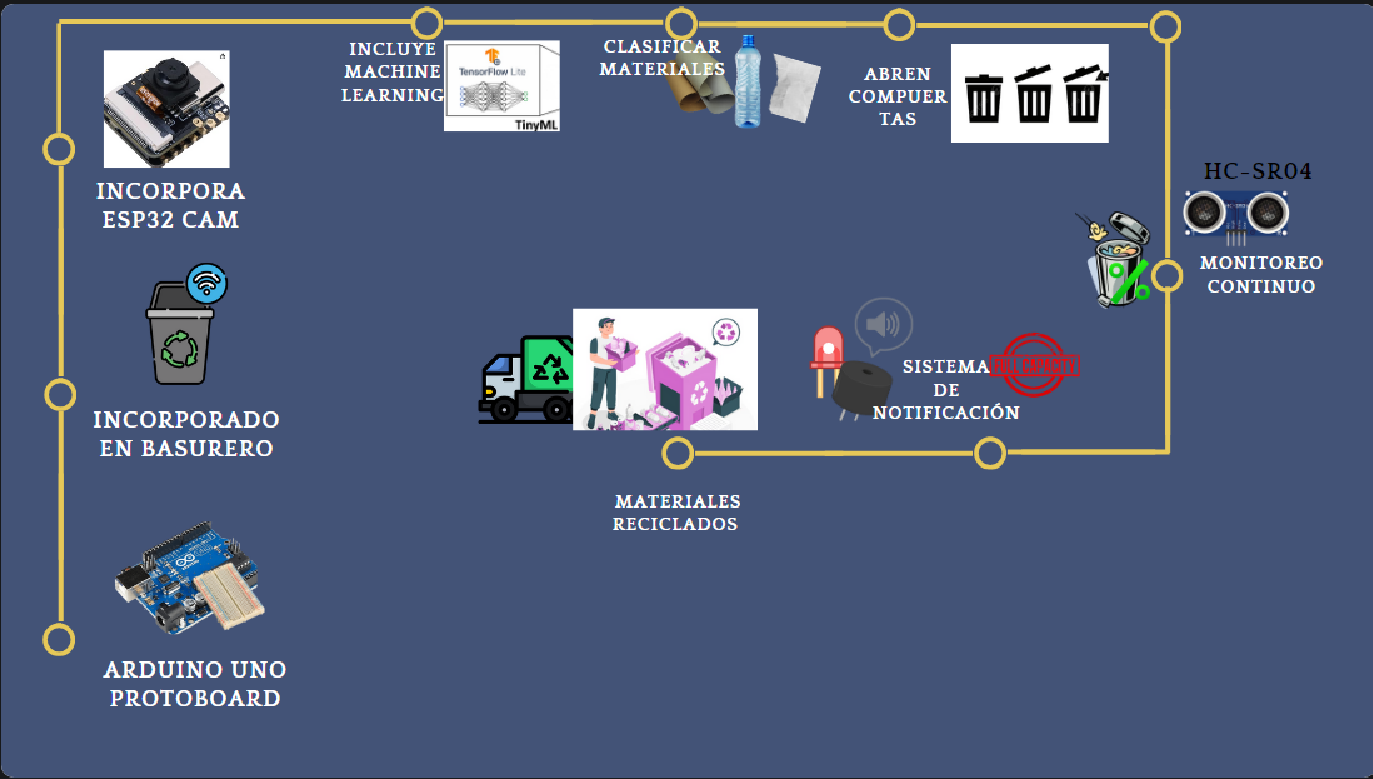
\includepdf{Imagenes/dc1.pdf}
\subsection{Descripción del diseño conceptual planteado}
\textbf{1. Arduino UNO R3}

El Arduino Uno es el corazón del sistema, encargado de recibir señales de los distintos componentes (cámara, sensores, etc.) y tomar decisiones en función de los datos recibidos.

Interacción: El Arduino coordina todo el sistema. Recibe las imágenes desde la cámara (ESP32 CAM), los datos de clasificación del modelo de machine learning (TinyML), y las lecturas del sensor ultrasónico (HC-SR04). Luego, controla la apertura de las compuertas y activa el sistema de notificación según sea necesario.

Acción: Procesa todas las señales y ejecuta comandos para manejar los actuadores y sensores.

\textbf{2. Incorporación de ESP32 CAM (Cámara)} 

La ESP32 CAM está instalada dentro del basurero. Su principal tarea es capturar imágenes de los residuos que se introducen. 

	\textbf{Interacción:} Cada vez que se coloca un objeto en el basurero, se activa la cámara para tomar una foto. Esta imagen es esencial para el siguiente paso, que es la clasificación mediante machine learning. 

	\textbf{3. Procesamiento con Machine Learning (TinyML)} 

Una vez que la cámara toma la imagen del residuo, esta se envía al sistema de machine learning, específicamente utilizando TensorFlow Lite, una versión ligera diseñada para dispositivos como la ESP32. 

    \textbf{Interacción:} El sistema de machine learning procesa la imagen en tiempo real y clasifica el material como plástico, papel, vidrio, etc. Esto se basa en el entrenamiento previo de un modelo que ha aprendido a identificar diferentes tipos de residuos. 

	\textbf{Decisión:} Dependiendo de la clasificación del material, el sistema decide en qué compartimiento debe depositarse el residuo. 

A continuación planteamos el siguiente diseño de como el modulo ESP32 CAM está involucrado de cierto modo con el proceso de machine Learning:


\begin{figure}[H]
	\centering
	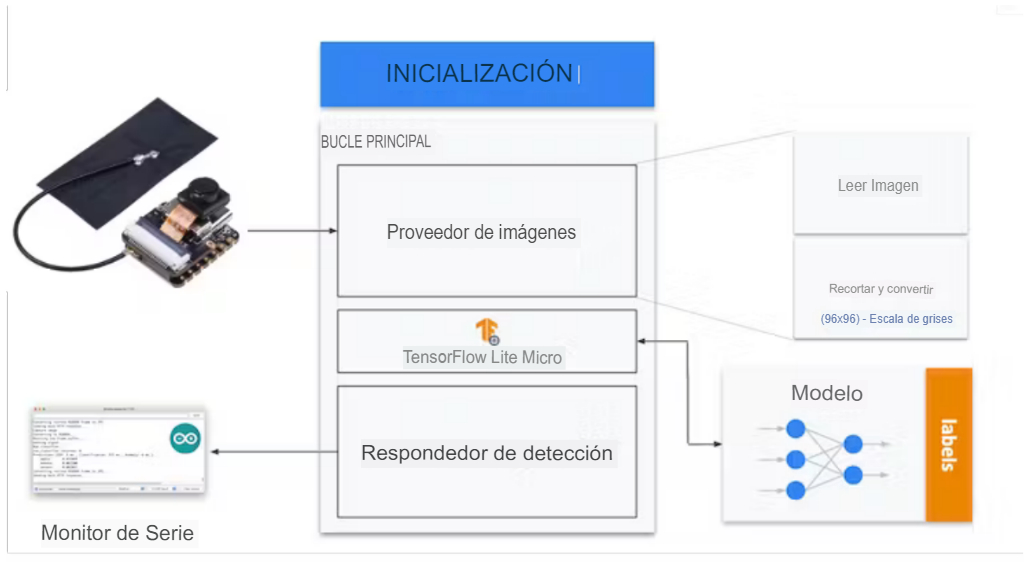
\includegraphics[scale  = 0.50]{Imagenes/ESP32-XIAO-CNN.jpg}
	\caption{ESP32 CAM y Machine Learning}{Fuente: Adaptado de~\cite{art_Xiao}}

\end{figure}

\textbf{Descripción}

\textbf{Inicialización}

Basicamente es configurar el sistema, inicializando todos los componentes del hardware y el software necesarios para realizar el procesamiento de imágenes y la clasificación.

Luego se inicializa la XIAO ESP32 CAM y el modelo de TensorFlow Lite Micro se carga en la memoria.

\textbf{Proveedor de Imágenes}

Función: La XIAO ESP32 CAM captura la imagen del objeto o material que se desea clasificar.

Proceso:

Cuando se le da una imagen a la cámara, su principal tarea es capturar la imagen y enviarla para ser procesada.

Leer Imagen: Se obtiene la imagen capturada en bruto.

Recortar y Convertir: Esta imagen es procesada, recortada y convertida a escala de grises para reducir la cantidad de datos y permitir una clasificación más eficiente. Aquí se menciona que la imagen se ajusta a una resolución de 96x96 píxeles.

\textbf{TensorFlow Lite Micro}

Función: Una vez que la imagen ha sido preprocesada, es enviada al módulo de TensorFlow Lite Micro, que está ejecutándose en la ESP32. Este módulo es responsable de aplicar el modelo de machine learning a la imagen procesada.

Proceso:
La imagen recortada y convertida es alimentada al modelo entrenado que reside en el sistema. Este modelo ha sido previamente entrenado para identificar ciertos patrones en las imágenes (clasificación de materiales, por ejemplo).

Modelo: El modelo de machine learning es una red neuronal simple, optimizada para sistemas embebidos con bajos recursos como la ESP32. El modelo toma como entrada la imagen convertida y devuelve una clasificación, basada en etiquetas predefinidas (labels) que corresponden a los materiales o categorías que el sistema debe reconocer.

\textbf{Respondedor de Detección}

Función: Una vez que el modelo ha procesado la imagen y ha generado una salida, el respondedor de detección se encarga de interpretar esta salida y tomar una acción en función de la predicción.

Proceso:
El sistema compara la salida del modelo con las etiquetas posibles (plástico, papel y cartón).

La respuesta de la detección (la etiqueta del material identificado) se envía al monitor serie para que podamos visualizarla.
Esto lo vamos a hacer por motivos de ver como se va comportando el modelo de detección y en base a eso, hacer ajustes o aplicar técnicas de optimizar.


El Arduino cuando lo conectemos puede utilizar esta salida para realizar una acción, como activar un motor para mover el residuo al compartimiento correspondiente o encender una señal de alerta.

\textbf{Monitor de Serie (Interfaz de Usuario)}

Función: El monitor de serie muestra las salidas del sistema, permitiendonos ver la clasificación en tiempo real.

Proceso:
A través de la consola de monitor serial, se pueden ver las etiquetas o categorías de los materiales clasificados.

Este componente puede también actuar como una herramienta de depuración, ayudando a entender cómo está funcionando el proceso en general.


	\textbf{4. Apertura de compuertas según la clasificación} 

Una vez que el machine learning ha clasificado el residuo, el sistema de control que viene siendo Arduino recibe la instrucción de abrir la compuerta correspondiente. 

    \textbf{Interacción:} El Arduino Uno controla motores o actuadores que abren las compuertas del basurero según el tipo de material identificado. Por ejemplo, si se detecta plástico, se abre la compuerta destinada para plásticos. 

	\textbf{Acción:} El residuo es depositado en el compartimiento adecuado para su recolección posterior. 

	\textbf{5. Monitoreo continuo del nivel de llenado (HC-SR04)} 

Mientras los residuos se van acumulando, el sensor ultrasónico HC-SR04 monitorea continuamente el nivel de llenado de cada compartimiento. 

    \textbf{Interacción:} Este sensor mide la distancia entre el residuo más alto y el sensor, que está colocado en la parte superior del compartimiento. A medida que los residuos se acumulan, el sensor detecta que la distancia se reduce, lo que indica que el compartimiento se está llenando. 

	\textbf{Decisión que va a tomar} Si el compartimiento alcanza un cierto nivel como "lleno", el sistema activará una alerta para indicar que se necesita vaciar el compartimiento(s). 

	\textbf{6. Sistema de notificación} 

El sistema incluye un mecanismo de notificación visual y/o sonora (buzzer y LEDs). Este se activa en dos situaciones principales: 

    \textbf{Llenado del compartimiento:} Cuando el sensor HC-SR04 detecta que un compartimiento está lleno, activa una señal para notificar que el basurero necesita ser vaciado. 

	\textbf{Error o evento inusual:} También puede notificar si se detecta algún material que no puede clasificarse, o si hay algún error en el proceso. 

	\textbf{Interacción:} El Arduino Uno controla las luces LED o el buzzer, emitiendo una alerta visual (como encender una luz roja) o sonora (emitir un pitido) cuando es necesario. 

	\textbf{7. Materiales reciclados y gestión de residuos} 

Los residuos clasificados correctamente son depositados en diferentes compartimientos dentro del basurero. 

    \textbf{Interacción:} Una vez que el material se clasifica y se deposita, el sistema de monitoreo continúa supervisando los niveles de llenado. Los materiales reciclados se almacenan hasta que un operador recoja los residuos para su tratamiento en una planta de reciclaje. 

	\newpage
\addcontentsline{toc}{chapter}{Bibliografía}
\begin{thebibliography}{99}

    \bibitem{mohd}
    \textit{Mohd Mahboob Ali, Harshavardhan CHVS, Gundumalla Sai Teja, B. Veera Jyothi,  L. Suresh Kumar. (2024). Intelligent waste sorting system: leveraging arduino for automated trash identification and categorization.} Disponible en: \url{https://cspub-ijcisim.org/index.php/ijcisim/article/view/733}

    \bibitem{jasim}
    \textit{Jasim, A. M., Qasim, H. H., Jasem, E. H., Saihood, R. H. (2021). An internet of things based smart waste system. International Journal of Electrical and Computer Engineering (IJECE), 11(3), 2577-2585.}

    \bibitem{anggrawan}
    \textit{Anggrawan, A., Hadi, S., Satria, C. (2022). IoT-Based garbage container system using NodeMCU ESP32 microcontroller. Journal of Advances in Information Technology Vol, 13(6).}

    \bibitem{pnud}
    \textit{G, C. a. G. (2024, July 24). PANAMÁ: DISPOSICIÓN y RECOLECCIÓN DE DESECHOS. RETOS DE UN NUEVO GOBIERNO. OPRA. } Disponible en: \url{https://observapanama.com/panama-disposicion-y-recoleccion-de-desechos-retos-de-un-nuevo-gobierno/}

    \bibitem{ecoembes}
    \textit{Ecoembes, «La tecnología del reciclaje, ¿ayuda al medioambiente? | Ecoembes», Ecoembes Reduce Reutiliza y Recicla.} Accedido: 10 de octubre de 2024. [En línea]. Disponible en: \url{https://reducereutilizarecicla.org/tecnologia-del-reciclaje/}
    
    \bibitem{caputo}
    \textit{G. Caputo, «Tecnología Sostenible ¿Qué es y cómo contribuye al desarrollo sostenible?», DoGood People.} Accedido: 10 de octubre de 2024. [En línea]. Disponible en: \url{https://www.dogoodpeople.com/es/tendencias-rsc/tecnologia-sostenible/tecnologia-sostenible-su-contribucion-desarrollo-sostenible/}
    
    \bibitem{microcontroladores}
    \textit{«Introduccion A Los Microcontroladores Pic», dokumen.pub.} Accedido: 10 de octubre de 2024. [En línea]. Disponible en: \url{https://dokumen.pub/introduccion-a-los-microcontroladores-pic.html}
    
    \bibitem{pena}
    \textit{C. Peña, Introducción a Arduino. RedUsers, 2020.}

    \bibitem{mecafenix}
    \textit{“Arduino ¿Que es, como funciona? y sus partes”. Ingeniería Mecafenix.} Accedido el 13 de octubre de 2024.\url{https://www.ingmecafenix.com/electronica/programacion/arduino/}

    \bibitem{delivery}
    \textit{ESP32 NodeMCU Módulo WLAN WiFi Junta de Desarrollo} \url{https://www.az-delivery.de/es/products/esp32-developmentboard}
    
    \bibitem{salvador}
    \textit{R. A. Salvador y C. B. Prieto, «Sistema de seguridad con reconocimiento facial en módulo ESP32», Mare Ingenii, vol. 4, n.o 1, Art. n.o 1, oct. 2022, doi: 10.52948/mare.v4i1.684.}

    \bibitem{foto_xiao}
    \textit{Seeed Studio XIAO ESP32S3 Sense}Accedido el 10 de octubre de 2024 \url{https://www.seeedstudio.com/XIAO-ESP32S3-Sense-p-5639.html}
    
    \bibitem{russo}
    \textit{C. Russo, H. Ramón, N. Alonso, B. Cicerchia, L. Esnaola, y J. P. Tessore, Tratamiento masivo de datos utilizando técnicas de machine learning. Universidad Nacional de Entre Ríos, 2016.} Accedido: 8 de octubre de 2024. [En línea]. Disponible en: \url{http://repositorio.unnoba.edu.ar/xmlui/handle/23601/107}
    
    \bibitem{betancourt}
    \textit{G. A. Betancourt, «LAS MÁQUINAS DE SOPORTE VECTORIAL (SVMs)», Sci. Tech., vol. 1, n.o 27, Art. n.o 27, abr. 2005.} Accedido: 8 de octubre de 2024. [En línea]. Disponible en: \url{https://revistas.utp.edu.co/index.php/revistaciencia/article/view/6895}

    \bibitem{udin}
    \textit{Sistema de monitoreo de acuicultura} Accedido el 10 de octubre de 2024.\url{https://humanizationoftechnology.com/sistema-de-monitoreo-de-acuicultura/revista/iot/05/2022/.}
    
    \bibitem{sinaluisa}
    \textit{I. F. Sinaluisa Lozano, C. A. Gallardo Naula, A. J. Morales Dominguez, y C. W. Montufar Paguay, «Internet de las Cosas aplicada a la movilidad y recolección inteligentes de residuos sólidos municipales», Polo Conoc. Rev. Científico - Prof., vol. 8, n.o 7 (JULIO 2023), pp. 944-961, 2023.}

    \bibitem{logic}
    \textit{Empresa Logix5 Smart Solutions S.L}Accedido el 10 de octubre de 2024\url{https://roboticaeducativa.logix5.com/}
    
    \bibitem{buying}
    \textit{M. Buying, «Contenedores de basura inteligentes: pioneros en una revolución en la gestión sostenible de residuos», Contenedores De Basura México.} Accedido: 8 de octubre de 2024. [En línea]. Disponible en: \url{https://contenedoresdebasura.com/contenedores-de-basura-inteligentes-pioneros-en-una-revolucion-en-la-gestion-sostenible-de-residuos/}
    
    \bibitem{quimbita}
    \textit{M. Quimbita y M. Andrés, «Evaluación de pasarela LoRa/LoRaWAN en entornos urbanos», oct. 2018.} Accedido: 8 de octubre de 2024. [En línea]. Disponible en: \url{https://riunet.upv.es/handle/10251/109791}

    \bibitem{chile}
    \textit{primer basurero “inteligente” de Chile en el centro de Santiago}Accedido el 10 de octubre de 2024 \url{https://www.plataformaurbana.cl/archive/2015/11/12/instalan-el-primer-basurero-inteligente-de-chile-en-el-centro-de-santiago/.}
    
    \bibitem{manrique}
    \textit{H. M. Manrique, «UNIVERSIDAD NACIONAL DEL CALLAO».}
    
    \bibitem{ali}
    \textit{M. M. Ali, H. Chvs, G. S. Teja, B. V. Jyothi, y L. S. Kumar, «Intelligent Waste Sorting System: Leveraging Arduino for Automated Trash Identification and Categorization», Int. J. Comput. Inf. Syst. Ind. Manag. Appl., vol. 16, n.o 3, Art. n.o 3, jul. 2024.}
    
    \bibitem{hassan}
    \textit{H. Hassan, F. Saad, y M. S. Mohd Raklan, «A Low-Cost Automated Sorting Recycle Bin powered by Arduino Microcontroller», en 2018 IEEE Conference on Systems, Process and Control (ICSPC), dic. 2018, pp. 182-186. doi: 10.1109/SPC.2018.8704146.}
    
    \bibitem{buitrago}
    \textit{D. A. Buitrago Aponte, «Sistema de clasificación de alimentos a través de inteligencia artificial: Estudio del tomate», may 2023.} Accedido: 8 de octubre de 2024. [En línea]. Disponible en: \url{https://hdl.handle.net/1992/73814}
    
    \bibitem{perez}
    \textit{I. H. Pérez-Tavera, «Arduino IDE», Vida Científica Bol. Científico Esc. Prep. No 4, vol. 11, n.o 21, Art. n.o 21, ene. 2023.}
    
    \bibitem{tollervey}
    \textit{N. H. Tollervey, Programming with MicroPython: Embedded Programming with Microcontrollers and Python. O’Reilly Media, Inc., 2017.}

    \bibitem{mpy}
    \textit{ESP32 MPY-Jama un nuevo entorno de desarrollo para Micropython | profe Tolocka} Accedido el 10 de octubre de 2024.\url{https://www.profetolocka.com.ar/2023/02/02/esp32-mpy-jama-un-nuevo-entorno-de-desarrollo-para-micropython/}
    
    \bibitem{red_neuronal}
    \textit{«Red neuronal convolucional», Wikipedia, la enciclopedia libre. 24 de mayo de 2024.} Accedido: 9 de octubre de 2024. [En línea]. Disponible en: \url{https://es.wikipedia.org/w/index.php?title=Red_neuronal_convolucional&oldid=160312860}
    
    \bibitem{vision_artificial}
    \textit{«Visión artificial», Wikipedia, la enciclopedia libre. 21 de julio de 2024.} Accedido: 9 de octubre de 2024. [En línea]. Disponible en: \url{https://es.wikipedia.org/w/index.php?title=Visi%C3%B3n_artificial&oldid=161428067}
    
    \bibitem{opencv}
    \textit{«OpenCV», Wikipedia, la enciclopedia libre. 14 de febrero de 2024.} Accedido: 9 de octubre de 2024. [En línea]. Disponible en: \url{https://es.wikipedia.org/w/index.php?title=OpenCV&oldid=158183931}
    
    \bibitem{numpy}
    \textit{«NumPy», Wikipedia. 30 de septiembre de 2024.} Accedido: 9 de octubre de 2024. [En línea]. Disponible en: \url{https://en.wikipedia.org/w/index.php?title=NumPy&oldid=1248522317}

    \bibitem{xiaotabla}
    \textit{DataSheet de XIAO ESP32 CAM}Disponible en: \url{https://www.seeedstudio.com/XIAO-ESP32S3-Sense-p-5639.html?queryID=be6f53c7ae317f6cbbc28f0668fb03df&objectID=5639&indexName=bazaar_retailer_products}
            
    \bibitem{ultrasonc}
    \textit{How the HC-SR04 Sensor Works and Example Programs with Arduino», NN Digital | Learn Arduino, ESP8266 / NodeMCU, STM32, Raspberry Pi, Microcontroller and Other Information Technology.} Accedido el 9 de octubre de 2024\url{https://www.nn-digital.com/en/blog/2019/08/07/how-the-hc-sr04-sensor-works-and-example-programs-with-arduino/}

    \bibitem{servo_motor}
    \textit{«Micro Servo Motor SG90 9g | Arduino.cl - Compra tu Arduino en Línea».} Accedido: 9 de octubre de 2024. [En línea]. Disponible en: \url{https://arduino.cl/producto/micro-servo-motor-sg90-9g/}

    \bibitem{link_miniservos}
    \textit{SIPYTOPF Paquete de Servomotores}. Accedido el 10 de octubre de 2024. \url{https://www.amazon.com/-/es/SIPYTOPF-Paquete-servomotores-Helic%C3%B3ptero-Caminar/dp/B09185SC1W/ref=sr_1_32?__mk_es_US=%C3%85M%C3%85%C5%BD%C3%95%C3%91&sr=8-32}.

    \bibitem{link_conectores_cables}
    \textit{BOJACK Conectores y Cables para Protoboard}. Accedido el 10 de octubre de 2024. \url{https://www.amazon.com/BOJACK-Solderless-Flexible-Breadboard-Connecting/dp/B08YRGVYPV/ref=mp_s_a_1_3?sr=8-3}.

    \bibitem{link_protoboard}
    \textit{MCIGICM Protoboard sin Soldadura}. Accedido el 10 de octubre de 2024. \url{https://www.amazon.com/MCIGICM-soldadura-bloques-conexi%C3%B3n-distribuci%C3%B3n/dp/B08115P2T4/ref=sr_1_2_sspa?__mk_es_US=%C3%85M%C3%85%C5%BD%C3%95%C3%91&crid=KKEKRCG6EY1X&dib=eyJ2IjoiMSJ9.n_ouM0H1-4UlTfT6NnyzOP27agXFvwpdpQDA9kKxVzYLIAPmmt34gPN84r3OHZayHjnz7fQt8U3TmlUkgyUJpWt_fMGmwHs2DcVvZUrXjoNGETKxSpBpJic-OuEVggA_lFd7uPpaGgGgm20KoLvvq30nabWY1ExK5I87qrsEqVxgn4BwJps4tvDKiF9VqoFEjmBz8p_EcKd_mvLJ7fmupow2SDy6tBmHZKkMvwW4xAo.SCKCgXJxXbckWRCMhoJUNEoTPZyXpXKILz-lFKFfMW0&dib_tag=se&keywords=2+protoboards&qid=1728768709&sprefix=2+protoboard%2Caps%2C139&sr=8-2-spons&sp_csd=d2lkZ2V0TmFtZT1zcF9hdGY&psc=1}.

    \bibitem{link_buzzer}
    \textit{Buzzer Piezoeléctrico para Proyectos Electrónicos}. Accedido el 10 de octubre de 2024. \url{https://www.amazon.com/piezoel%C3%A9ctricos-electr%C3%B3nico-computadoras-componentes-electr%C3%B3nicos/dp/B07VK1GJ9X/ref=sxin_16_pa_sp_search_thematic_sspa?__mk_es_US=%C3%85M%C3%85%C5%BD%C3%95%C3%91&cv_ct_cx=buzzer&sbo=RZvfv%2F%2FHxDF%2BO5021pAnSA%3D%3D&sr=1-5-6024b2a3-78e4-4fed-8fed-e1613be3bcce-spons&sp_csd=d2lkZ2V0TmFtZT1zcF9zZWFyY2hfdGhlbWF0aWM&psc=1}.

    \bibitem{link_arduino}
    \textit{Placa Elegoo ATmega328P Arduino UNO}. Accedido el 10 de octubre de 2024. \url{https://www.amazon.com/Elegoo-Placa-ATmega328P-ATMEGA16U2-Arduino/dp/B01EWOE0UU/ref=sxin_16_pa_sp_search_thematic_sspa?__mk_es_US=%C3%85M%C3%85%C5%BD%C3%95%C3%91&cv_ct_cx=arduino+uno&s=electronics&sbo=RZvfv%2F%2FHxDF%2BO5021pAnSA%3D%3D&sr=1-1-6024b2a3-78e4-4fed-8fed-e1613be3bcce-spons&sp_csd=d2lkZ2V0TmFtZT1zcF9zZWFyY2hfdGhlbWF0aWM&psc=1}.

    \bibitem{art_Xiao}
    \textit{MJRoBot (Marcelo Rovai). “TinyML Made Easy: Image Classification w/ XIAO ESP32S3 Sense”.}Accedido el 10 de octubre de 2024.\url{https://www.hackster.io/mjrobot/tinyml-made-easy-image-classification-w-xiao-esp32s3-sense-cb42ae}
    
\end{thebibliography}

\end{document}
